%Original version in April 2002 by Antje Endemann
%
%Adapted for usage in Student Conference course by jubo (050118).
%Optimized for usage with pdflatex. For usage with plain latex,
%figures must be in Postscript (.ps or .eps files) and additional
%packages must be imported.
%Last updated 100105 by jubo
%
%This template works for outline and annotated bibliography
%(deliverable 2) without any changes.
%For usage with full and final papers (deliverables 3 and 4a/b)
%you must make several changes. All necessary changes are
%described in three specific commented sections preceded by
%`%%%%% BEGIN OF ADJUSTMENTS SECTION %%%%%'.
%The changes are in order of appearance:
%   - adjust the `\documentclass' command
%   - uncomment the abstract section
%   - adjust the `\bibliographystyle' command

%%%%% BEGIN OF 1st ADJUSTMENTS SECTION %%%%%
% You must use only one of the following `\documentclass' commands
% For the outline and annotated bibliography (deliverable 2)
% you must use the following command:
%
% \documentclass[runningheads,a4paper,oribibl]{llncs}
%
% For the full and final paper (deliverables 3 and 4a/b)
% you must use the command below (and put the one above in comments).
% In other words, the 'oribib' option must be used for Deliverable 2
% but not for 3 and 4a/b.
% 
%
\documentclass[runningheads,a4paper]{llncs}
%
%%%%% END OF 1st ADJUSTMENTS SECTION %%%%%

\usepackage[T1]{fontenc}  %% needed for special characters (umlaut)
\usepackage[utf8]{inputenc}
\usepackage{graphicx}     %% for graphical things such as including pictures
\usepackage{url}          %% for proper formatting of URLs

\begin{document}

\pagestyle{headings}

\mainmatter

% \title{Guidelines for Designing Touch Interfaces for Controlling Robotic Nozzles in Critical Emergency Situations.}

\title{Can a high color contrast touch interface increase user reaction time when using a smart phone web based application.}

% response
% reaction time

% The abbreviated title will be shown in the headers of even pages.
% You should use the full title unless it is too long.

% \titlerunning{Touch Interfaces for Robotic Nozzles in Emergency Situations}

\titlerunning{Can high color contrast increase user reaction time}

\author{Albin Hübsch}

\institute{
	Department of Computing Science \\
	Umeå University, Sweden \\
	\email{id11ahh@cs.umu.se}
}

\maketitle

%%%%% BEGIN OF 2nd ADJUSTMENTS SECTION %%%%%
% Do NOT include an abstract in the outline and annotated bibliography
% (deliverable 2). For the full and final paper (deliverables 3 and 4a/b),
% you must uncomment the following two commands and place your text for
% the abstract in between them.
%
\begin{abstract}
Here goes paper abstract
\end{abstract}
%
%%%%% END OF 2nd ADJUSTMENTS SECTION %%%%%

\section{Introduction}
The main goal with this paper is to evaluate if color contrast has a significant impact on usability in web based smart-phone applications. Consumer touch screen devices such as smart-phones has rapidly increased in amount and availability recent years. The touch screen technology have made great advances ~\cite{jennings2013touch} and it is more frequently used as a way of receiving user input. When this technology moves to a broader audience, higher demands on usability needs to be set~\cite{gong2004guidelines}. To further explore how usability can be improved using touch screen technology we are in this paper investigating if reaction time (referred to as RT in this paper) and user input errors (referred to as IE in this paper) can reach better results by increasing color contrast within the interface. Earlier work done in this field are exploring how we perceive different color contrast and how it can affect our reading performance~\cite{wu2003improving}. It has also been proved that Chromaticity, Contrast, and Cone Opponency in color space can affect RTs~\cite{mckeefry2003simple}. Many best practices for Mobile development also shows that "requirements for sufficient color contrast"~\cite{marcus2013design} must be meet to best exaggerate the content. But still the question remains, if a high color contrast interface can increase the the RT\footnote{Reaction time: the time it takes for a user to react on instructions} and decrease user IE\footnote{Input errors: the number of user input errors when interacting with a system}.

High RTs and low user IE are especially desirable when designing user interfaces for situations with high demands on quick user input and low error tolerance such as emergency situations. The results of this paper can be used by any designer or developer.

\section{Method}
In order to be able to test if color contrast has an substantial impact on the RT and user IE of a touch user interface we have designed a simple web application for an Android smart-phone. The application exists in two versions, one with low color (LC) contrast and one with high color contrast (HC) as can be seen in Fig~\ref{fig:application}.

\begin{figure}
	\centering
	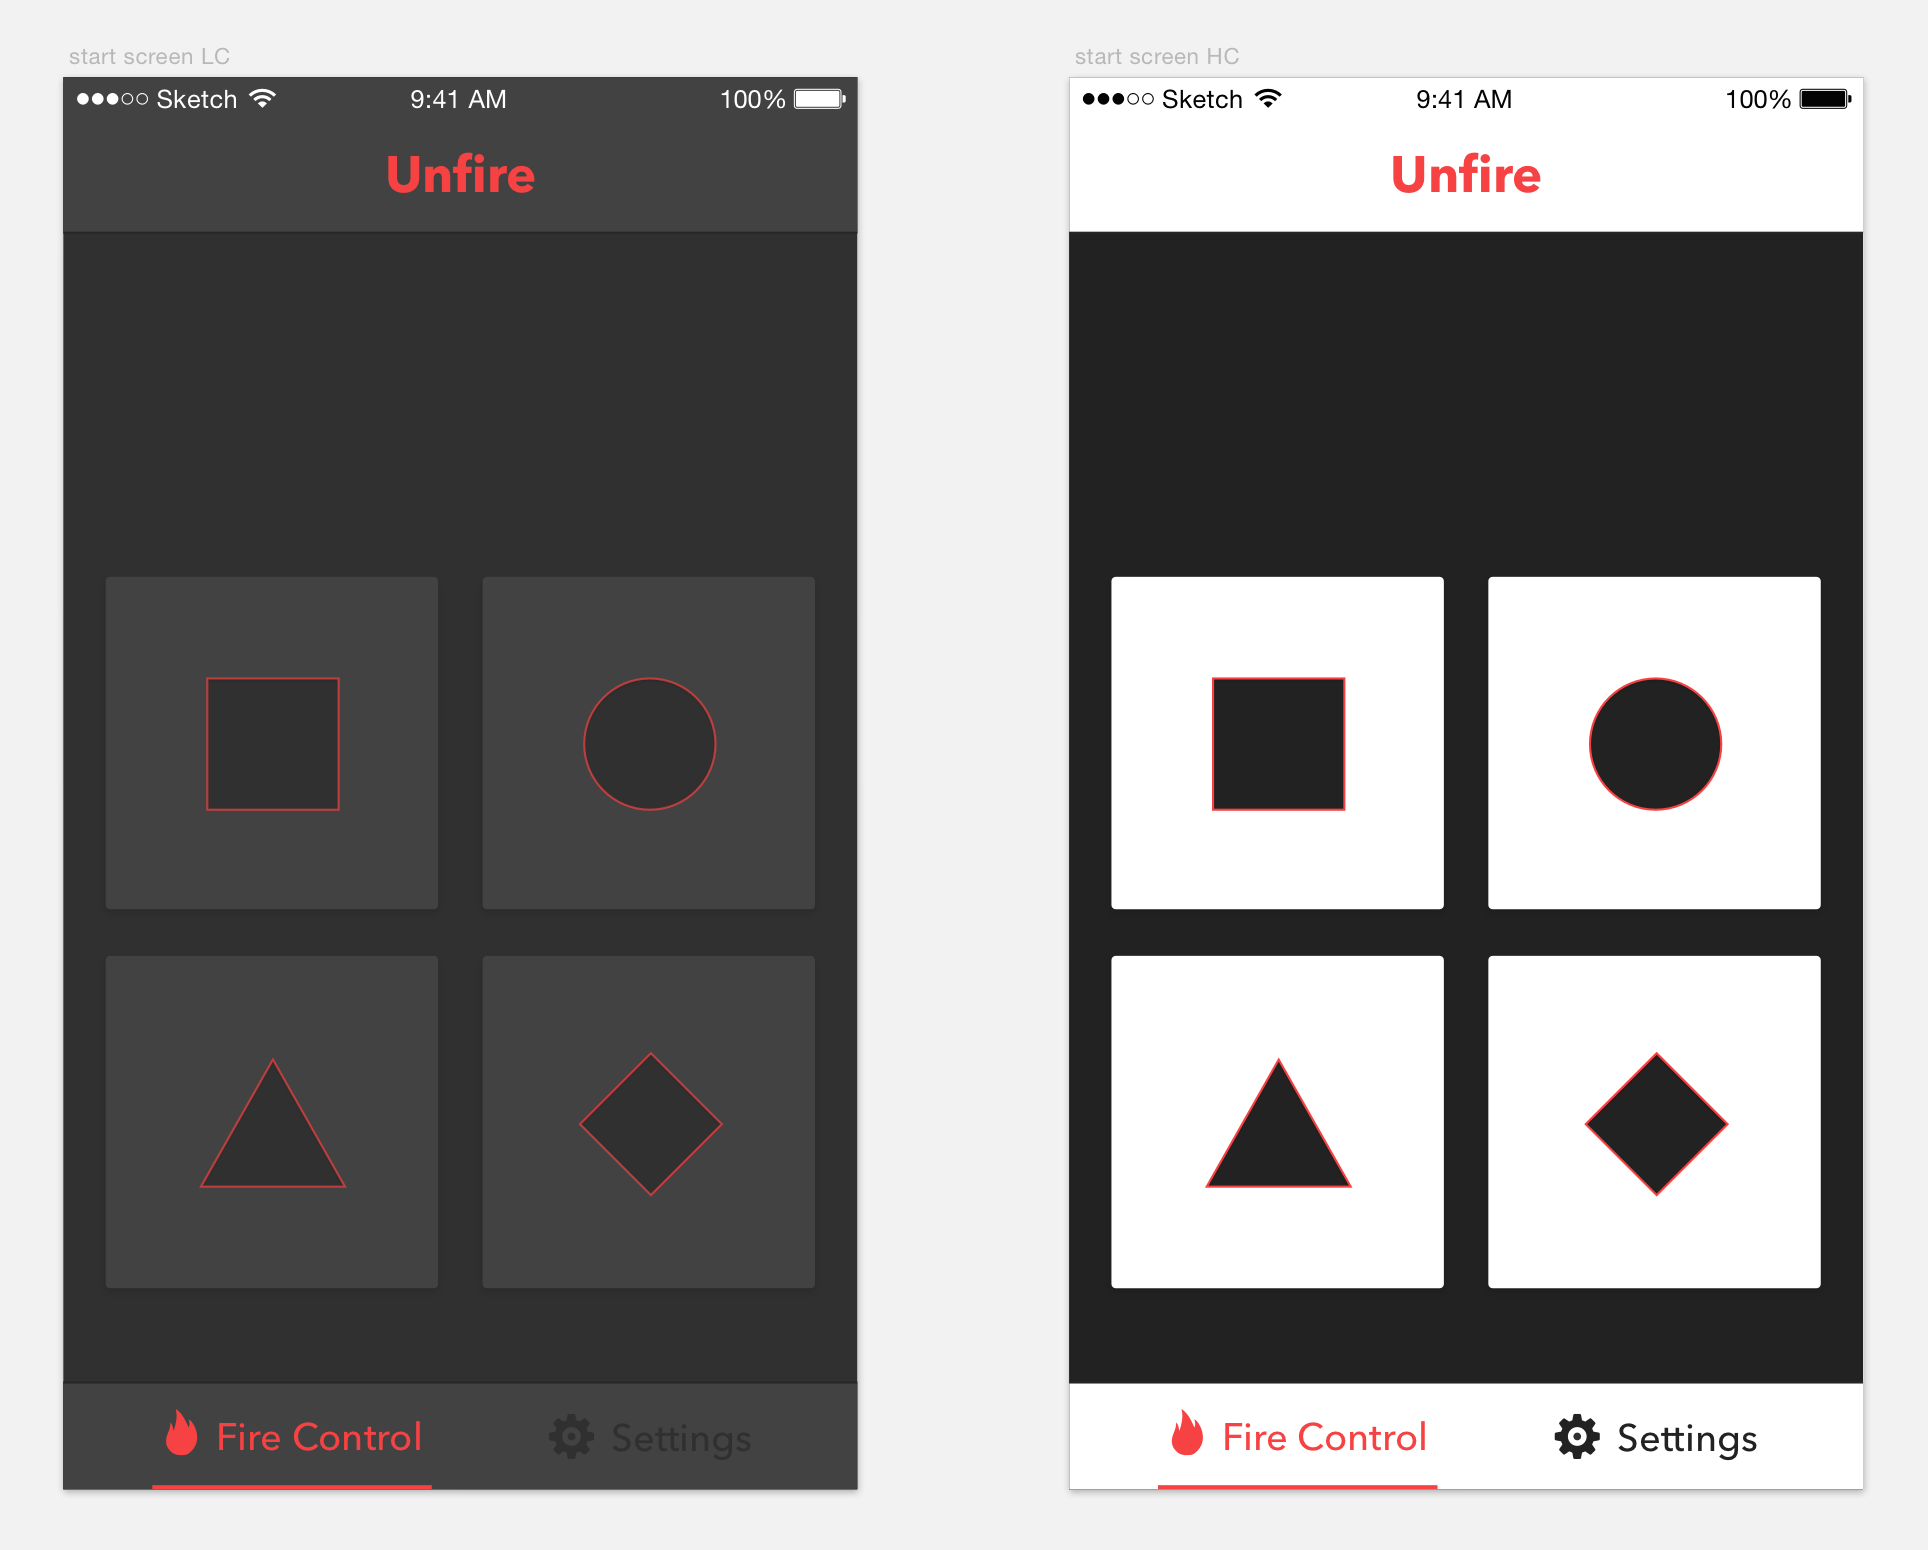
\includegraphics[width=\textwidth]{application}
	\caption{Our two color contrast versions of our application designed.\label{fig:application}}
\end{figure}

We designed the application by following design guidelines given here~\cite{hoober2011designing} and~\cite{johnson2013designing}. 

\subsection{Designing the A/B test}
We conducted an A/B test to measure the differences in RT and IE between the two versions. An A/B test is a commonly used method by developers and designers to test differences in performance between applications when the differentiated factors are known~\cite{johnson2013designing}. As in this case our known factor is the contrast difference. 

The application consists of 4 buttons~\footnote{On screen button}, each button representing a function. To fraction each button from the others we put a unique shape in each button. The shapes we used are a, square, circle, triangle and a rhomb~\ref{fig:application}.

To be able to give the test persons consistent instructions through the complete test we designed a program that presented the instructions on a secondary screen. The instructions were a series of shapes equally to the shapes in the application buttons and the test persons where told to press the representative shape in the application as fast as they could to measure the reaction time. If they pressed the wrong button they where told to continue the test by pressing the right button, the application registered this as an IE. Each test were performed indoors with varying surroundings such as different lightning conditions and noise levels. We tested each version of the application on 5 persons all within the same age group (20-30) and with a variety of backgrounds. We had a gender split of 50\% women and 50\% men. In total we got 10 test results that we later analyzed against each other to measure if any differences in RTs or IEs between the two versions could be statistically confirmed.

\subsection{Evaluation of the A/B test}
Our test data received from the tests consisted of UNIX timestamps~\footnote{\url{http://www.unixtimestamp.com/}} in milliseconds. Each time the user interacted with the application it registered which button that was pressed and saved it together with a UNIX timestamp. Equally, every time the instruction program showed a new symbol it logged that together with a UNIX timestamp. As a result we received two data sets of symbols with corresponding timestamps for each test person, resulting in a total of approximately 400 records. Although the data were hard to interpret due to its compact look, a pyhton program were written to clean it up. We calculated each difference (RT) in time between when the instruction were given and when user interaction registered. Out of this we could calculate the mean RT for both groups LC and HC. The calculation of RT did not take in consideration if user input were a no match. We still considered it as an reaction.

IEs were counted every time the user pressed a non matching object compared to the one given in the instructions. All IEs in each group, LC and HC, were counted to see if one of the groups produced more IEs.

\section{Result}
From our results we can not draw any statistically significant differences in RT between the two groups HC and LC. This is most probably due to corrupt test data, a result from limitations in web application technology, see section \ref{sec:discussion}. With the IEs we found a significant difference between the groups.

\subsection{Reaction Times (RT)}
asd

\subsection{Input Errors}
asd

\section{Discussion} \label{sec:discussion}
In this section we will discuss the results from the tests. We will discuss what the results mean and how they should and could be interpreted. We are currently in the stage of analyzing our data.

\subsection{Drawbacks and Limitations} \label{subsec:drawbacks}
One of the main drawbacks of this study is the limited number of test subjects. In order to get more credible result a larger group of test persons should be included. Preferable we should also had let the test persons do the test several of times to eliminate possible surrounding factors that could have affect the results. 

Below is a asd
\begin{description}
	\item[Our group of test subjects is to small] To be able to get a more statistical valid result the test group has to be bigger.
	\item[Many affecting parameters] The prototype is simple in its appearance but there are still many parameters that can affect the users interaction and their RTs. Icons, icon size, optimal number of soft-buttons, size of hand-held device etc. All this, and more, should have been researched and taken into account if done again. 
	\item[Limited test environment] Our tests were made with using an Android smart-phone~\footnote{OnePlus two \url{https://oneplus.net/2}} system and the application were done using HTML5 and CSS3. We can not surely imply, without testing, that the same results would appear on an iPhone or any other smart-phone.
\end{description}

\subsection{Future Work}
Due to limited time given for this paper there are things that could be improved or just continued to be worked on. We have some concrete suggestions that could be a case for future work.

\begin{itemize}
	\item Extend the test group with more test subjects. It is possible to think that the patterns that slightly appeared in our results will appear even more significant with a larger group of test subjects.
	\item Our collected test data can be downloaded and used freely to investigate other aspect not mentioned in this paper. One proposal is to look at the different shapes and try to detect possible error patterns between them. Is the rhomb more frequently pressed wrongly compared to the other shapes?
	\item Does our results apply on other systems and techniques? Our tests are limited to the Android system and a web application solution. It remains to answer if our results applies on all other systems. This is also a way of isolate some of all the affecting parameters mentioned in~\ref{subsec:drawbacks}.
\end{itemize}

%%%%% BEGIN OF 3rd ADJUSTMENTS SECTION %%%%%
% For the outline and annotated bibliography (deliverable 2)
% you must use the following two commands:
%
\nocite{*}  % Includes ALL entries from the .bib-file, even if they are
            % not '\cite{}'-ed in the text above
% \bibliographystyle{plain-annote}
%
% For the full and final paper (deliverables 3 and 4a/b)
% use ONLY the following commands (i.e. put the commands above into
% comments and uncomment the command below):
%
\bibliographystyle{splncs}
%
%%%%% END OF ADJUSTMENTS SECTION %%%%%

\bibliography{Bibliography}

\end{document}
